\documentclass[11pt,a4paper]{article}
\usepackage[T1]{fontenc}
\usepackage[utf8]{inputenc}
\usepackage{lmodern,microtype}
\usepackage[margin=28mm,headheight=14pt]{geometry}
\usepackage{amsmath,amssymb,amsthm,mathtools,bm}
\usepackage{booktabs,array,longtable,enumitem,xcolor,fancyhdr,graphicx}
\usepackage{placeins}
\usepackage{hyperref,xurl}
\definecolor{inkblue}{HTML}{163D58}
\definecolor{linkteal}{HTML}{126C75}
\hypersetup{colorlinks=true,linkcolor=inkblue,citecolor=linkteal,urlcolor=linkteal,
pdftitle={Sharp Late Coefficients and Borel Continuation of Resonant Lambert Inverses},
pdfauthor={Research contribution prepared for the ProveIt project}}
\pagestyle{fancy}\fancyhf{}
\fancyhead[L]{\small\textsc{Resonant Lambert inverses}}
\fancyhead[R]{\small Late coefficients and Borel continuation}
\fancyfoot[C]{\thepage}
\setlength{\parskip}{4pt}
\setlength{\parindent}{14pt}
\setlist{itemsep=3pt,topsep=5pt}
\numberwithin{equation}{section}
\newtheorem{theorem}{Theorem}[section]
\newtheorem{proposition}[theorem]{Proposition}
\newtheorem{lemma}[theorem]{Lemma}
\newtheorem{corollary}[theorem]{Corollary}
\theoremstyle{definition}
\newtheorem{definition}[theorem]{Definition}
\theoremstyle{remark}
\newtheorem{remark}[theorem]{Remark}
\newcommand{\C}{\mathbb C}
\newcommand{\R}{\mathbb R}
\newcommand{\Q}{\mathbb Q}
\newcommand{\Z}{\mathbb Z}
\newcommand{\N}{\mathbb N}
\newcommand{\dd}{\,\mathrm d}
\newcommand{\ii}{\mathrm i}
\newcommand{\Li}{\operatorname{Li}}
\newcommand{\Disc}{\operatorname{Disc}}
\newcommand{\Cat}{\operatorname{Cat}}
\newcommand{\Res}{\operatorname{Res}}
\newcommand{\borel}{\mathcal B}
\newcommand{\SU}{\mathcal S}
\newcommand{\F}{\mathcal F}
\newcommand{\ord}{\operatorname{ord}}
\newcommand{\re}{\operatorname{Re}}
\newcommand{\im}{\operatorname{Im}}
\newcommand{\smallO}{\mathcal O}
\newcommand{\coef}[2]{[#1^{#2}]}
\allowdisplaybreaks[2]
\begin{document}
\hypersetup{pageanchor=false}
\begin{titlepage}
\centering
\vspace*{15mm}
{\color{linkteal}\large\textsc{Polylogarithms $\boldsymbol\cdot$ Transseries}}\par
\vspace{11mm}
{\color{inkblue}\LARGE\bfseries Sharp Late Coefficients and\par
\vspace{3mm}Borel Continuation of\par
\vspace{3mm}Resonant Lambert Inverses\par}
\vspace{9mm}
{\large Hyperbolic amplitudes, uniform reversion,\par
and the two nearest arithmetic actions\par}
\vspace{12mm}
{Prepared for Vladimir Reshetnikov and the ProveIt project\par}
\vspace{3mm}
{12 October 2026\par}
\vspace{12mm}
\begin{minipage}{0.91\textwidth}
\begin{abstract}
We resolve the explicit late-coefficient conjecture in the incoming report
\emph{Double Resonance and Nested Stokes Geometry in Polylogarithmic Lambert
Inversion}. Its resonant forward tail has only one odd coefficient, whereas
nonlinear inversion creates every odd sector. We prove the predicted
$\cosh(\pi^2u)$ and $\sinh(\pi^2u)$ amplitudes by a uniform factorial-convolution
estimate, give the first inverse-index correction, and retain uniformity as
the slow parameter $u$ tends to zero. A finite-phase version identifies the
linear forward coefficient as the quantity that dresses the leading action
amplitudes. The two Borel endpoints admit explicit logarithmic models with a
continuous remainder; after the first correction, dilogarithms give a model
with a continuously differentiable remainder. A separate application of
Sauzin's nonlinear resurgence theorems proves continuation outside
$4\pi^2\Z$ and summability away from the real directions. We specify which
claims are new calculations, which are applications of established theory,
and which questions remain open. Exact finite checks and reproducible
numerical diagnostics accompany the proofs.
\end{abstract}
\end{minipage}
\vfill
\begin{minipage}{0.91\textwidth}\small
\textbf{Research status.} Conventional mathematical proofs and executed
computational checks. This is an unrefereed research contribution prepared
with ChatGPT assistance. Global publication priority and proof-assistant
formalization are not claimed. The source snapshot and precise integration
updates are recorded in Section~\ref{sec:audit}.
\end{minipage}
\end{titlepage}
\pagenumbering{roman}
\hypersetup{pageanchor=true}
\begingroup
\small
\setlength{\parskip}{0pt}
\tableofcontents
\endgroup
\clearpage
\pagenumbering{arabic}
\section{The problem and the contribution}\label{sec:setting}

Let $d(m)$ be the number of positive divisors of $m$. The resonant Lambert
function
\begin{equation}\label{eq:F}
 \F(t)=\sum_{m\ge1}\frac{d(m)}m e^{-mt}
       =\sum_{a\ge1}\frac{\Li_1(e^{-at})}{a},\qquad \re t>0,
\end{equation}
is a direct bridge between the two programs named in the research request.
It is a superposition of polylogarithms, but its expansion at $t=0$ has a
factorially divergent tail. Inverting its large logarithmic core produces
ordinary exponential sectors with a second, much smaller, exponential scale
inside their Stokes discontinuity.

The incoming manuscript \cite{incoming} obtains an exact finite formula for
the inverse-sector coefficients and proves their Borel radius. Its
Section~11.1, equations labelled \texttt{eq:conj-even} and
\texttt{eq:conj-odd}, leaves the leading coefficient amplitudes conjectural.
This article proves those formulas and their first correction. It also
answers the continuation part of the next research question, Section~11.2,
by checking the hypotheses of an established nonlinear resurgence theorem.

\subsection{Notation and the two independent variables}

Throughout, put
\begin{equation}\label{eq:constants}
 A=4\pi^2,\qquad c=\frac A4=\pi^2,\qquad
 d=\frac{A^2}{288}=\frac{\pi^4}{18},\qquad
 b_n=\frac{\Gamma(n)}n\quad(n\ge1).
\end{equation}
The lower-case constant $d$ in \eqref{eq:constants} has no argument and is
distinct from the divisor function $d(m)$. Define the formal series
\begin{equation}\label{eq:R}
 R(t)=\sum_{n\ge1}r_nt^n,\qquad
 r_1=-\frac14,\quad
 r_n=\begin{cases}
 4b_nA^{-n}\zeta(n)^2,&n\ge2\text{ even},\\
 0,&n\ge3\text{ odd}.
 \end{cases}
\end{equation}
The central object is the unique formal solution
\begin{equation}\label{eq:implicit}
 V(q,u)+\frac u2 V(q,u)^2+uR\bigl(qe^{-V(q,u)}\bigr)=0,
 \qquad V(q,u)=\sum_{n\ge1}C_n(u)q^n.
\end{equation}
Here $q$ and $u$ are independent variables: $q$ is the sector variable and
$u$ is the slow parameter. The equality is an identity of formal series,
not an evaluation of the divergent series $R$.

To recover the physical inverse, write
\begin{equation}\label{eq:physical}
 C_* =\frac{\zeta(2)}2-\gamma^2-2\gamma_1,
 \quad X=\sqrt{2(Y-C_*)},\quad u=X^{-1},\quad q=e^{\gamma-X},
 \quad t=qe^{-V}.
\end{equation}
The positive square root is used for large real $Y$. The constant
$\gamma_1$ uses the convention
$\zeta(1+s)=s^{-1}+\gamma-\gamma_1s+O(s^2)$.
The actual inverse of \eqref{eq:F} has \eqref{eq:implicit} as its formal
sector expansion under \eqref{eq:physical}. Large coefficient index $n$ and
large target $Y$ are different limits; our uniform estimates make their
interaction explicit.

\subsection{The resolved conjecture}

For $\epsilon\in\{0,1\}$ set
\[
 H_0(z)=\cosh z,\qquad H_1(z)=\sinh z,
\]
and let a prime denote differentiation with respect to $z$.

\begin{theorem}[Sharp uniform late coefficients]\label{thm:main}
For every $U>0$, uniformly for complex $|u|\le U$ as $n\to\infty$,
\begin{align}
 \frac{(-1)^{n+1}A^nC_n(u)}{4ub_n}
 &=H_{n\bmod2}(z)+\frac{K_{n\bmod2}(u)}n
      +O_U(n^{-2}),\qquad z=cu,\label{eq:main-expansion}\\
 K_\epsilon(u)
 &=\left(du+\frac{1+u}{2}z^2\right)H_\epsilon(z)
       +(2+u)zH_\epsilon'(z).\label{eq:K}
\end{align}
The quotient at $u=0$ is removable. For odd $n$, the error term on the
right of \eqref{eq:main-expansion} is in fact $O_U(|u|n^{-2})$.

In particular, uniformly for every real $0<u\le U$,
\begin{align}
 C_{2m}(u)
 &=-\frac{4u\Gamma(2m)}{2mA^{2m}}\cosh(Au/4)
       \{1+O_U(m^{-1})\},\label{eq:even-main}\\
 C_{2m+1}(u)
 &=\frac{4u\Gamma(2m+1)}{(2m+1)A^{2m+1}}\sinh(Au/4)
       \{1+O_U(m^{-1})\}.\label{eq:odd-main}
\end{align}
No lower bound on $u$ is required.
\end{theorem}

The leading amplitudes in \eqref{eq:even-main}--\eqref{eq:odd-main} are the
precise conjecture in \cite{incoming}. The estimate, its moving-parameter
scope, and \eqref{eq:K} strengthen that conjecture. Sections~\ref{sec:leading}
and \ref{sec:correction} supply elementary coefficient proofs.
They do not rely on a Borel continuation hypothesis.

The second principal result is analytic.

\begin{theorem}[Borel radius and continuation]\label{thm:analytic-preview}
For every fixed $u\in\C\setminus\{0\}$, the shifted Borel transform
\begin{equation}\label{eq:BorelV}
 \widehat V_u(\xi)=\sum_{n\ge1}\frac{C_n(u)}{\Gamma(n)}\xi^{n-1}
\end{equation}
has radius exactly $A$, with genuine singularities at both $A$ and $-A$.
Its principal germ admits analytic continuation along every path beginning
at the origin and thereafter avoiding $A\Z$. The formal series $V(q,u)$
is $1$-summable in each direction not congruent to $0$ or $\pi$ modulo
$2\pi$. For $u=0$ both $V$ and its Borel transform vanish.
\end{theorem}

The continuation assertion is an application of Sauzin's theorems
\cite{Sauzin2015}, after a specific change of coordinates that we prove in
Section~\ref{sec:continuation}. It determines an allowed singularity set;
it does not assert that every lattice point is singular on every sheet.
Section~\ref{sec:Borel} gives explicit boundary models involving logarithms
and dilogarithms, with a continuously differentiable remainder.

\subsection{Relationship to existing work}

The forward Lambert family and its resurgent arithmetic structure are
established work of Dorigoni--Kleinschmidt and Broadhurst--Dorigoni
\cite{DK2021,BD2026}. The present paper studies the late coefficients of a
specific nonlinear inverse. The starting coefficient formula, polynomial
signs, Catalan degree, and exact forward Stokes jump belong to the incoming
report \cite{incoming}; we reproduce short derivations where they make
this paper self-contained.

The mechanism of one large factorially weighted component has substantial
antecedents. Bender--Richmond studied rapidly growing Lagrange coefficients
\cite{BR1984}; Borinsky developed a complete algebra for factorial
coefficient asymptotics, including composition and inversion
\cite{Borinsky2018}. In our input the two equal-modulus contributions
$A^{-n}$ and $(-A)^{-n}$ coexist. We therefore do not apply a theorem for a
single positive action without checking the additional phase structure.
Our proof works directly with the finite Lagrange sum and supplies the
uniform bound missing from the source conjecture. The finite-phase theorem
in Section~\ref{sec:phases} records the same calculation in reusable form.

The novelty claimed here is scoped: a resolved project conjecture, explicit
first corrections and Borel boundary formulas for this model, a uniform
extension to a vanishing slow parameter, and a checked application of
nonlinear resurgence that answers a stated continuation question.
Worldwide priority for each model-specific formula has not been established.

\section{The forward expansion and the exact reversion formula}\label{sec:forward}

\subsection{How a sum of polylogarithms acquires factorial coefficients}

For $t>0$, every summand in \eqref{eq:F} is positive and has negative
derivative. Normal convergence on compact subsets of $\re t>0$ proves
holomorphy, and monotonicity gives a positive real inverse. The Mellin
representation is
\begin{equation}\label{eq:mellin}
 \F(t)=\frac1{2\pi\ii}\int_{\sigma-\ii\infty}^{\sigma+\ii\infty}
       \Gamma(s)\zeta(1+s)^2t^{-s}\dd s,\qquad \sigma>0.
\end{equation}
It follows by Mellin inversion of $e^{-mt}$ and the absolutely convergent
Dirichlet identity $\sum d(m)m^{-1-s}=\zeta(1+s)^2$.

At $s=0$ the integrand has a triple pole. Multiplication of the Laurent
series of $\Gamma(s)$ and $\zeta(1+s)$ yields the residue
\[
 \frac12(\log(1/t)+\gamma)^2+C_*.
\]
The residue at $s=-n$ is
\begin{equation}\label{eq:r-residue}
 r_n=\frac{(-1)^n}{n!}\zeta(1-n)^2.
\end{equation}
The zeta functional equation gives \eqref{eq:R}; standard special-function
conventions follow \cite{DLMF}. In particular $r_2=1/288$,
and every odd coefficient after $r_1$ vanishes at a trivial zeta zero.
Shifting the Mellin contour by any fixed number of poles gives the usual
finite-order asymptotic expansion
\begin{equation}\label{eq:forward-asym}
 \F(t)\sim\frac12(\log(1/t)+\gamma)^2+C_*+R(t),
 \qquad t\to0^+.
\end{equation}
Only finitely many terms are asserted at each remainder order. The
factor $\Gamma(n)/n$ in \eqref{eq:R} proves that $R$ has radius zero.

Substituting \eqref{eq:physical} in \eqref{eq:forward-asym} and cancelling
$X^2/2+C_*$ gives
$XV+V^2/2+R(qe^{-V})=0$, which is \eqref{eq:implicit} after division by $X$.
This calculation explains both the quadratic feedback and the exponential
composition; neither is introduced as an arbitrary test equation.

\subsection{Formal existence and a finite coefficient formula}

\begin{proposition}[Exact finite reversion]\label{prop:lagrange}
Equation~\eqref{eq:implicit} has a unique solution in $q\Q[u][[q]]$.
For $1\le k\le n$, define
\begin{equation}\label{eq:T}
 T_{n,k}(u)=\sum_{j=0}^{k-1}\binom{k-1}{j}
      n^{k-1-j}(k)_j\left(\frac u2\right)^j,
\end{equation}
where $(k)_j=k(k+1)\cdots(k+j-1)$ and $(k)_0=1$. Then
\begin{equation}\label{eq:C-finite}
 C_n(u)=-\sum_{k=1}^{n}\frac{u^k}{k!}[q^n]R(q)^k\,T_{n,k}(u).
\end{equation}
\end{proposition}
\begin{proof}
The coefficient of $V$ at $q=V=0$ is $1$, so coefficient recursion gives
formal existence and uniqueness over $\Q[u]$. To obtain the displayed
formula, insert an auxiliary variable $\eta$ and write
\[
 V=-\eta u\,\frac{R(qe^{-V})}{1+uV/2}.
\]
Formal Lagrange inversion in $\eta$ gives
\[
 V=\sum_{k\ge1}\frac{(-\eta u)^k}{k!}
 \left.\partial_v^{k-1}
 \bigl(R(qe^{-v})^k(1+uv/2)^{-k}\bigr)\right|_{v=0}.
\]
Only $k\le n$ contributes to $q^n$, making $\eta=1$ a legitimate
coefficientwise specialization. Since
$[q^n]R(qe^{-v})^k=e^{-nv}[q^n]R(q)^k$, Leibniz' rule turns the derivative
into $(-1)^{k-1}T_{n,k}(u)$. This proves \eqref{eq:C-finite}.
\end{proof}

\begin{proposition}[Signs, valuations, and the first coefficients]
\label{prop:structure}
For all $n\ge1$,
\begin{align}
 &(-1)^{n+1}C_n(u)\in\Q_{\ge0}[u]\setminus\{0\},\label{eq:sign}\\
 &\deg C_n=2n-1,\qquad
 [u^{2n-1}]C_n=\frac{(-1)^{n+1}\Cat_{n-1}}{2^{3n-1}},\label{eq:degree}\\
 &\ord_{u=0} C_n=
 \begin{cases}1,&n=1\text{ or }n\text{ even},\\2,&n\ge3\text{ odd}.
 \end{cases}\label{eq:valuation}
\end{align}
For odd $n\ge3$, $[u^2]C_n=n r_{n-1}/4$. Explicitly,
\begin{align}
 C_1(u)&=\frac u4,\nonumber\\
 C_2(u)&=-\frac u{288}-\frac{u^2}{16}-\frac{u^3}{32},\label{eq:firstC}\\
 C_3(u)&=\frac{u^2}{384}+\frac{7u^3}{288}
              +\frac{3u^4}{128}+\frac{u^5}{128}.\nonumber
\end{align}
\end{proposition}
\begin{proof}
In any nonzero monomial contributing to $[q^n]R^k$, the number of linear
factors has the parity of $n$. Hence $(-1)^n[q^n]R^k\ge0$, and all
coefficients of $T_{n,k}$ are nonnegative. The top degree comes only from
$k=n$, $j=n-1$, using $r_1^n=(-1/4)^n$; evaluation gives
\eqref{eq:degree}. The linear coefficient is $-r_n$. For odd $n\ge3$, the
quadratic coefficient is
$-n[q^n]R^2/2=-n(2r_1r_{n-1})/2=n r_{n-1}/4>0$.
The displayed first polynomials follow from \eqref{eq:C-finite}.
These structural facts were proved in \cite{incoming}; the proof is included
because the exact valuations are essential to uniformity at $u=0$.
\end{proof}

\section{Uniform factorial convolution and the hyperbolic amplitudes}
\label{sec:leading}

The source conjecture correctly identifies the contribution of any fixed
number of factors in \eqref{eq:C-finite}. The missing step is to control
that number uniformly. A factorial convolution estimate supplies this
control without fitting late coefficients or assuming resurgence.

\subsection{A majorant that retains the endpoint factorial}

Scale the coefficients by
\begin{equation}\label{eq:positive-scaled}
 a_m=A^m(-1)^mr_m,\qquad a_1=c,\qquad
 a_{2j}=4b_{2j}\zeta(2j)^2,\qquad a_{2j+1}=0\ (j\ge1),
\end{equation}
and set
\begin{equation}\label{eq:S-D}
 S_{n,k}=[x^n]\left(\sum_{m\ge1}a_mx^m\right)^k,
 \qquad D_n(u)=(-1)^{n+1}A^nC_n(u).
\end{equation}
All $a_m$ are nonnegative. If
$K\ge\max\{c,4\zeta(2)^2\}$, then $a_m\le Kb_m$ for every $m$.
Equation~\eqref{eq:C-finite} becomes
\begin{equation}\label{eq:D-formula}
 D_n(u)=\sum_{k=1}^n\frac{u^k}{k!}S_{n,k}T_{n,k}(u).
\end{equation}

\begin{lemma}[Endpoint-preserving factorial bounds]\label{lem:factorial}
For $n\ge2$,
\begin{equation}\label{eq:b-convolution}
 \sum_{m=1}^{n-1}b_mb_{n-m}\le3b_{n-1}.
\end{equation}
Consequently, for $1\le k\le n$,
\begin{equation}\label{eq:S-bound}
 S_{n,k}\le K^k3^{k-1}b_{n-k+1},\qquad
 \frac{n^{k-1}b_{n-k+1}}{b_n}\le ke^k.
\end{equation}
\end{lemma}
\begin{proof}
The ratio of the $m$th summand in \eqref{eq:b-convolution} to $b_{n-1}$ is
\[
 \frac{n-1}{m(n-m)}\binom{n-2}{m-1}^{-1}
 \le\binom{n-2}{m-1}^{-1}.
\]
For $N\ge2$ every interior binomial coefficient $\binom Nj$ is at least
$N$, so
$\sum_{j=0}^N\binom Nj^{-1}\le2+(N-1)/N<3$.
The cases $N=0,1$ satisfy the same bound. This proves
\eqref{eq:b-convolution}. Induction on $k$, shifting the convolution index
at each step, gives
$[x^n](\sum_{m\ge1}b_mx^m)^k\le3^{k-1}b_{n-k+1}$, and therefore the first
part of \eqref{eq:S-bound}.

For the second part let $h=k-1$. Direct factorial cancellation gives
\begin{equation}\label{eq:ratio-exact}
 \frac{n^hb_{n-h}}{b_n}
 =\frac{n}{n-h}\prod_{i=1}^h\left(1-\frac in\right)^{-1}.
\end{equation}
The first factor is at most $k$, since $(k-1)(n-k)\ge0$.
For the increasing function $f(x)=-\log(1-x)$,
\[
 \sum_{i=1}^{k-1}f(i/n)
 \le n\int_0^{k/n}f(x)\dd x
 =k+(n-k)\log(1-k/n)\le k.
\]
At $k=n$ the integral is finite and $0\log0$ is interpreted as zero.
Exponentiation proves the bound, including the endpoint $k=n$.
\end{proof}

For $|u|\le U$, the exact polynomial \eqref{eq:T} satisfies
\begin{equation}\label{eq:T-bound}
 |T_{n,k}(u)|\le n^{k-1}(1+U)^{k-1},
\end{equation}
because $(k)_j\le(2n)^j$. Combining this with Lemma~\ref{lem:factorial}
gives the central estimate
\begin{equation}\label{eq:master-majorant}
 \frac1{b_n}\left|\frac{u^k}{k!}S_{n,k}T_{n,k}(u)\right|
 \le \frac{k}{k!}K^k3^{k-1}e^kU^k(1+U)^{k-1}
 \le \frac{kB_U^k}{k!}
\end{equation}
for a suitable fixed $B_U$. The final majorant is summable in $k$ and
independent of $n$. It removes the spurious $e^{O(\sqrt n)}$ loss of the
coarser composition count in the predecessor.

The same conclusion holds after division by $u$ for even $n$, and by
$u^2$ for odd $n\ge3$. In the latter case the exact sum begins at $k=2$,
by \eqref{eq:valuation}. On a compact disk one uses
$|u|^{k-v}\le\max(1,U)^k$, with $v=1$ or $2$. Every quotient is a
polynomial, so no estimate divides by a small nonzero number.

\subsection{The contribution of one large index}

\begin{lemma}[First endpoint extraction]\label{lem:endpoint}
For $k\ge2$ and $n\ge k+2$,
\begin{equation}\label{eq:endpoint}
 S_{n,k}=k c^{k-1}a_{n-k+1}+E_{n,k},\qquad
 0\le E_{n,k}\le6\binom{k}{2}K^k3^{k-2}b_{n-k}.
\end{equation}
For $k=1$ the main term is exact.
\end{lemma}
\begin{proof}
Compositions with exactly one part greater than $1$ give the main term.
Every remaining composition has two parts at least $2$. Mark a pair of
such positions and use a union bound over $\binom{k}{2}$ choices.

For $N\ge4$,
\begin{equation}\label{eq:interior-b}
 \sum_{m=2}^{N-2}b_mb_{N-m}\le6b_{N-2}.
\end{equation}
Indeed, put $M=N-4$ and $j=m-2$. The ratio of a summand to $b_{N-2}$ is
\[
 \frac{M+2}{M+1}
 \frac{(j+1)(M-j+1)}{(j+2)(M-j+2)}\binom Mj^{-1}
 \le2\binom Mj^{-1}.
\]
The reciprocal-binomial bound proves \eqref{eq:interior-b}.
After summing the two marked parts, convolve with the remaining $k-2$
parts and enlarge the index range. The result is bounded by
\[
 6K^k[x^{n-2}]\left(\sum_{m\ge1}b_mx^m\right)^{k-1}
 \le6K^k3^{k-2}b_{n-k}.
\]
Summing over the marked pair proves \eqref{eq:endpoint}.
\end{proof}

For fixed $k$, multiplication of the remainder in \eqref{eq:endpoint} by
$n^{k-1}/b_n$ gives $O_k(n^{-1})$. The main index is $m=n-k+1$.
If $m$ is even, then
$n^{k-1}a_m/b_n\to4$; if $m$ is odd it is eventually zero.
Also $T_{n,k}(u)/n^{k-1}\to1$ locally uniformly in $u$.
Thus the limit of the $k$th summand in \eqref{eq:D-formula}, divided by
$b_n$, is
\begin{equation}\label{eq:fixed-k-limit}
 \frac{4k u^kc^{k-1}}{k!}
 =4u\frac{(cu)^{k-1}}{(k-1)!}
\end{equation}
when $n-k+1$ is even, and zero in the other parity.
The majorant \eqref{eq:master-majorant} now justifies summation of these
limits. Even $n$ selects even $k-1$ and produces $\cosh(cu)$; odd $n$
selects odd $k-1$ and produces $\sinh(cu)$.

\subsection{Uniform errors, including the zero-parameter boundary}

\begin{theorem}[A quantified proof of the source conjecture]
\label{thm:leading-rate}
For every $U>0$, uniformly for complex $|u|\le U$,
\begin{align}
 \frac{A^nC_n(u)}{4b_nu}&=-\cosh(cu)+O_U(n^{-1})
       &&(n\text{ even}),\label{eq:leading-even}\\
 \frac{A^nC_n(u)}{4b_nu^2}&=\frac{\sinh(cu)}u+O_U(n^{-1})
       &&(n\ge3\text{ odd}).\label{eq:leading-odd}
\end{align}
All quotients at $u=0$ are interpreted by continuity.
\end{theorem}
\begin{proof}
Split the finite sum at $k=n/2$ and first take $k\le n/2$. Let
$h=k-1$ and $R_{n,k}=n^hb_{n-h}/b_n$. The logarithm of
\eqref{eq:ratio-exact} and $-\log(1-x)\le2x$ on $[0,1/2]$ give
\begin{align}
 0\le\log R_{n,k}&\le\frac{h(h+3)}n,\nonumber\\
 |R_{n,k}-1|&\le\frac{ke^kh(h+3)}n,\label{eq:ratio-rate}\\
 \frac{n^hb_{n-h-1}}{b_n}
 &=R_{n,k}\frac{n-h}{(n-h-1)^2}
 \le\frac{4ke^k}{n}\quad(n\ge4).\nonumber
\end{align}
The last estimate controls \eqref{eq:endpoint}. Using the sharper
$(k)_j\le(2k)^j$ in \eqref{eq:T} gives
\begin{equation}\label{eq:T-rate}
 \left|\frac{T_{n,k}(u)}{n^h}-1\right|
 \le(1+kU/n)^h-1
 \le\frac{k^2U}{n}(1+U)^k.
\end{equation}
For the even endpoint $m=n-k+1\ge n/2$, the error
$\zeta(m)^2-1=O(2^{-m})$ is uniformly $O(n^{-1})$.
Combining these estimates bounds the difference between each normalized
summand and \eqref{eq:fixed-k-limit} by
\[
 \frac1n\frac{P(k)\widetilde B_U^k}{k!}
\]
for a fixed polynomial $P$. The bound also holds after division by the
valuation factor $u$ or $u^2$, as explained after
\eqref{eq:master-majorant}. It is summable over $k$.

For $k>n/2$ both the exact summands and the limiting exponential summands
have a majorant of the form $kB_U^k/k!$. The inequality $1\le2k/n$ makes
the summed tail $O_U(n^{-1})$. More generally, using
$1\le(2k/n)^M$ makes this tail $O_{U,M}(n^{-M})$ for any fixed $M$.
Summing \eqref{eq:fixed-k-limit} with its parity restriction proves
\eqref{eq:leading-even}--\eqref{eq:leading-odd}.
\end{proof}

For real $0\le u\le U$, one has $\cosh(cu)\ge1$ and
$\sinh(cu)/u\ge c$, including the limiting value at zero. Dividing by
these lower bounds proves the uniform relative versions
\eqref{eq:even-main}--\eqref{eq:odd-main}. This is stronger than an estimate
whose constant depends on a fixed lower bound for $u$.

\begin{corollary}[Two limits may be taken together]\label{cor:moving-u}
Let $u_n>0$, $u_n\to0$, and $n\to\infty$ through the indicated parity.
Then
\begin{equation}\label{eq:small-u-late}
 C_n(u_n)\sim
 \begin{cases}
 -4u_n b_nA^{-n},&n\text{ even},\\
 A u_n^2 b_nA^{-n},&n\text{ odd}.
 \end{cases}
\end{equation}
The rate at which $u_n$ approaches zero is unrestricted.
\end{corollary}
\begin{proof}
Apply the uniform relative bounds and use
$\cosh(cu)=1+O(u^2)$ and $\sinh(cu)=cu\{1+O(u^2)\}$.
\end{proof}

The coefficient theorem therefore applies to the physical slow parameter
$u=1/X$ while the sector index increases. It does not assert that the
divergent infinite sector series may be summed ordinarily at that physical
pair, nor does a coefficient estimate alone determine an optimally
truncated remainder of the actual inverse.

\section{Finite phases and changes of the initial coefficients}\label{sec:phases}

The hyperbolic functions reflect the two phases $1$ and $-1$ in the
forward coefficients. The same proof yields a finite-phase transformation
law, with no positivity requirement.

\begin{theorem}[Leading amplitudes for finitely many phases]
\label{thm:finite-phases}
Let $A>0$, $b_n=\Gamma(n)/n$, and
$\widetilde R(t)=\sum_{n\ge1}\widetilde r_nt^n$, with
$\widetilde r_1=\rho\in\C$. Suppose that for a finite set
$E\subset\{\omega\in\C:|\omega|=1\}$ of distinct phases,
\begin{equation}\label{eq:phase-input}
 |\widetilde r_n|\le K A^{-n}b_n,\qquad
 \frac{A^n\widetilde r_n}{b_n}
 =\sum_{\omega\in E}\kappa_\omega\omega^n+O(n^{-1}).
\end{equation}
Let $\widetilde C_n(u)$ be the coefficients of the zero-constant formal
solution of \eqref{eq:implicit} with $R$ replaced by $\widetilde R$.
Then, locally uniformly for $u\in\C$,
\begin{equation}\label{eq:phase-output}
 \widetilde C_n(u)=-u A^{-n}b_n
 \left\{\sum_{\omega\in E}\kappa_\omega\omega^n
                   e^{A\rho u/\omega}+O_U(n^{-1})\right\}.
\end{equation}
The bracketed formulation extends through $u=0$. Its error corresponds to
an absolute $O_U(|u|A^{-n}b_n/n)$ error in $\widetilde C_n$.
\end{theorem}
\begin{proof}
Apply the exact formula \eqref{eq:C-finite} to the new input and scale by
$A^n$. The first endpoint is now
$k(A\rho)^{k-1}(A^{n-k+1}\widetilde r_{n-k+1})$.
All remainder estimates of Lemmas~\ref{lem:factorial} and
\ref{lem:endpoint} apply to absolute values: the positivity assumption
was used to construct a majorant, not to establish an identity.
For $k\le n/2$, the remainder in \eqref{eq:phase-input} is $O(n^{-1})$
at the endpoint. The same proof as Theorem~\ref{thm:leading-rate} therefore
justifies the uniform $k$ summation with error $O_U(n^{-1})$.
For each phase the limiting sum is
\[
 -\sum_{k\ge1}\frac{u^k}{(k-1)!}(A\rho)^{k-1}
                 \kappa_\omega\omega^{n-k+1}
 =-u\kappa_\omega\omega^n e^{A\rho u/\omega}.
\]
The sum over $E$ is finite, which proves \eqref{eq:phase-output}.
\end{proof}

The action corresponding to $\omega$ is $\lambda_\omega=A/\omega$.
Its leading amplitude is multiplied by $e^{\lambda_\omega\rho u}$.
This multiplier comes entirely from repeated linear factors of the
forward series. The terms of $T_{n,k}$ with $j\ge1$, which encode the
quadratic part of the inverse core, enter one inverse-index order later.
Cancellation between distinct phases can occur on subsequences, so
\eqref{eq:phase-output} is an additive expansion. A relative equivalent
requires a separate nonvanishing argument.

\begin{corollary}[Polynomial changes of the forward tail]
\label{cor:prefix}
For the Lambert input, replace $R(t)$ by $R(t)+P(t)$, where $P(0)=0$ is a
fixed polynomial and $p_1=[t]P(t)$. The late coefficient formula is
\begin{equation}\label{eq:prefix}
 \widetilde C_n(u)=-2uA^{-n}b_n
 \left\{e^{A(p_1-1/4)u}+(-1)^n e^{-A(p_1-1/4)u}
                     +O_U(n^{-1})\right\}.
\end{equation}
In particular, changes satisfying $P(t)=O(t^2)$ leave both leading action
amplitudes unchanged.
\end{corollary}
\begin{proof}
A polynomial changes no sufficiently late forward coefficient. Apply
Theorem~\ref{thm:finite-phases} with $E=\{1,-1\}$ and
$\kappa_1=\kappa_{-1}=2$.
\end{proof}

This corollary gives a useful separation of data: the arithmetic tail
locates the leading actions, the linear term changes their amplitudes,
and the quadratic term first appears in the correction computed next.

\section{The first inverse-index correction}\label{sec:correction}

The leading amplitude only sees one large forward index and the linear
indices accompanying it. At the next order, a single quadratic forward
index also contributes. We retain that contribution uniformly in the number
of factors, then compute the corrections from the gamma ratios and from
$T_{n,k}$. This proves the full statement of Theorem~\ref{thm:main}.

\subsection{Two endpoint terms with a uniform remainder}

Recall the scaled coefficients and convolution coefficients from
Section~\ref{sec:leading}:
\[
 a_m=A^m(-1)^m r_m,\qquad
 S_{n,k}=[x^n]\left(\sum_{m\ge1}a_mx^m\right)^k.
\]
In particular $a_1=c$, $a_2=d$, and every $a_m$ is nonnegative. It is
convenient to shift the index once:
\begin{equation}\label{eq:alpha-shift}
 \alpha_j=a_{j+1},\qquad
 \alpha(x)=\sum_{j\ge0}\alpha_jx^j,\qquad
 S_{n,k}=[x^{n-k}]\alpha(x)^k.
\end{equation}
Thus $\alpha_0=c$, $\alpha_1=d$, and there is a constant $B$ such that
\begin{equation}\label{eq:alpha-bound}
 0\le\alpha_j\le B\Gamma(j)\qquad(j\ge1).
\end{equation}
Indeed $a_{j+1}=4\Gamma(j+1)\zeta(j+1)^2/(j+1)$ when $j+1$ is even,
and it is zero otherwise. The ratio $j/(j+1)$ is at most one, and
$\zeta(j+1)\le\zeta(2)$.

\begin{lemma}[The second endpoint contribution]\label{lem:second-endpoint}
There is a constant $B_*>0$ such that, whenever $n\ge12$ and
$1\le k\le n/2$,
\begin{equation}\label{eq:two-endpoints}
 \begin{split}
 S_{n,k}={}&kc^{k-1}a_{n-k+1}
       +k(k-1)c^{k-2}d\,a_{n-k}\\
       &\quad+O\bigl(B_*^k\Gamma(n-k-2)\bigr).
 \end{split}
\end{equation}
The second term is understood to be zero for $k=1$, and the implied
constant is independent of both $n$ and $k$.
\end{lemma}
\begin{proof}
We first record two elementary estimates. The sequence $F_j=j!$ satisfies
$F*F\le3F$ coefficientwise. For $M\ge1$, division of its $M$th convolution
coefficient by $M!$ gives
\[
 \sum_{j=0}^{M}\binom{M}{j}^{-1}\le3:
\]
the endpoints contribute two, and each of the $M-1$ interior terms is at
most $1/M$. The case $M=0$ is immediate. Iteration, followed by the change
$j_i\mapsto j_i-1$, gives
\begin{equation}\label{eq:positive-gamma-convolution}
 \sum_{\substack{j_1+\cdots+j_h=N\\j_i\ge1}}
       \prod_{i=1}^{h}\Gamma(j_i)
 \le3^{h-1}\Gamma(N-h+1),\qquad N\ge h\ge1.
\end{equation}

Removing the endpoints from the two-factor convolution gives a sharper
estimate:
\begin{equation}\label{eq:interior-gamma-convolution}
 \sum_{j=2}^{N-2}\Gamma(j)\Gamma(N-j)
       \le4\Gamma(N-2),\qquad N\ge4.
\end{equation}
For completeness, put $M=N-2$ and divide the left side by $M!$. The
result is $\sum_{i=1}^{M-1}\binom{M}{i}^{-1}$. For $M\ge3$, its two extreme
terms contribute $2/M$, and each of the remaining $M-3$ terms is at most
$2/[M(M-1)]$. The sum is at most $4/M$. The case $M=2$ also satisfies this
bound, proving \eqref{eq:interior-gamma-convolution}.

Now put $N=n-k$, so $N\ge k$ and $N\ge6$, and expand $\alpha(x)^k$
according to the number $h$ of positive indices. The case $h=1$ contributes
$kc^{k-1}\alpha_N$. For $h=2$, the indices $1,N-1$ and $N-1,1$ contribute
\[
 2\binom{k}{2}c^{k-2}\alpha_1\alpha_{N-1}
       =k(k-1)c^{k-2}d\alpha_{N-1}.
\]
By \eqref{eq:alpha-bound} and \eqref{eq:interior-gamma-convolution}, the
remaining $h=2$ terms are bounded by
$4\binom{k}{2}c^{k-2}B^2\Gamma(N-2)$.
For $h\ge3$, \eqref{eq:positive-gamma-convolution} bounds the contribution
by
\[
 \binom{k}{h}c^{k-h}B^h3^{h-1}\Gamma(N-h+1).
\]
Since $N\ge k\ge h$, one has
$\Gamma(N-h+1)\le\Gamma(N-2)$. The binomial theorem therefore bounds
the sum of all these remainders by $B_*^k\Gamma(N-2)$ after a fixed
increase of $B_*$. Substituting $\alpha_N=a_{n-k+1}$ and
$\alpha_{N-1}=a_{n-k}$ proves \eqref{eq:two-endpoints}.
\end{proof}

\subsection{The two elementary expansions}

The next estimates are uniform over the full range $k\le n/2$; their
constants may grow exponentially in $k$, because the Lagrange factor
$1/k!$ makes that growth summable. Define
\[
 Q_{n,k}(u)=n^{1-k}T_{n,k}(u),\qquad
 \beta_k=\frac{(k-1)(k+2)}2.
\]
For $|u|\le U$, the finite sum \eqref{eq:T} gives
\begin{equation}\label{eq:T-first-correction}
 Q_{n,k}(u)=1+\frac{k(k-1)u}{2n}
       +O_U\left(\frac{(1+k)^4e^{B_Uk}}{n^2}\right).
\end{equation}
To justify the uniform remainder, use
$\binom{k-1}{j}\le k^j/j!$ and $(k)_j\le(2k)^j$. The sum of the absolute
values of the terms with $j\ge2$ is at most
\[
 \sum_{j\ge2}\frac{(Uk^2/n)^j}{j!}
 \le\frac{U^2k^4}{2n^2}e^{Uk^2/n}.
\]
The inequality $k^2/n\le k/2$ proves
\eqref{eq:T-first-correction}. It also gives a bound
$|Q_{n,k}(u)|\le e^{Uk/2}$ that will be used for the endpoint remainder.

For the first endpoint, put $p=n-k+1$. When $p$ is even,
\begin{equation}\label{eq:gamma-first-correction}
 \frac{n^{k-1}a_p}{b_n}
 =4\left\{1+\frac{\beta_k}{n}
       +O\left(\frac{(1+k)^4e^{B_1k}}{n^2}\right)\right\};
\end{equation}
when $p$ is odd it is zero. The exact gamma ratio before multiplication
by $4\zeta(p)^2$ is
\begin{equation}\label{eq:gamma-ratio-exact}
 \frac{n^{k-1}b_{n-k+1}}{b_n}
 =\frac{n^k}{(n-k+1)\prod_{j=1}^{k-1}(n-j)}.
\end{equation}
Its logarithm equals $\beta_k/n+O(k^3/n^2)$: the offsets in the
denominator are $k-1,1,\ldots,k-1$, whose sum is $\beta_k$, and every
offset divided by $n$ is at most $1/2$. More explicitly,
$-\log(1-v)=v+O(v^2)$ uniformly for $0\le v\le1/2$. The logarithm
itself is $O(k^2/n)=O(k)$, so exponentiating introduces a remainder
$O((1+k)^4e^{B_1k}/n^2)$. Finally
$\zeta(p)^2=1+O(2^{-p})$, with $p\ge n/2$, and this exponentially small
error is absorbed by the displayed bound. This proves
\eqref{eq:gamma-first-correction}.

The second endpoint has the corresponding estimate
\begin{equation}\label{eq:gamma-second-endpoint}
 \frac{n^{k-1}a_{n-k}}{b_n}
 =\frac4n+O\left(\frac{(1+k)^2e^{B_2k}}{n^2}\right)
       \quad\text{if }n-k\text{ is even},
\end{equation}
and it is zero otherwise. Here the exact gamma ratio is
\[
 \frac{n^{k-1}b_{n-k}}{b_n}
 =\frac{n^k}{(n-k)\prod_{j=1}^{k}(n-j)}.
\]
Factor out $1/n$ and apply the same logarithmic estimate to the offsets
$k,1,\ldots,k$. This proves \eqref{eq:gamma-second-endpoint}.

The remainder in Lemma~\ref{lem:second-endpoint} is also uniformly of
second order after normalization. For $n\ge12$ and $k\le n/2$,
\begin{equation}\label{eq:endpoint-normalized-error}
 \frac{n^{k-1}\Gamma(n-k-2)}{b_n}
 =\frac{n^k\Gamma(n-k-2)}{\Gamma(n)}
 \le\frac{3^{k+2}}{n^2}.
\end{equation}
Indeed, the denominator ratio contains $k+2$ factors $n-j$, each at least
$n-k-2\ge n/3$. Combining
\eqref{eq:two-endpoints}--\eqref{eq:endpoint-normalized-error}, all errors
in the $k$th summand of \eqref{eq:C-finite}, after division by $b_n$ and
scaling by $A^n$, are bounded by
\begin{equation}\label{eq:summable-second-error}
 \frac{|u|}{n^2}\frac{M_U^k(1+k)^M}{k!},
\end{equation}
for constants $M_U$ and a fixed integer $M$. One obtains this bound by
leaving one factor $|u|$ outside and replacing the remaining
$|u|^{k-1}$ by $U^{k-1}$. Thus the estimates remain uniform after division
by $u$, with the removable value at zero.

\subsection{Summing the corrections}

We now complete the proof of Theorem~\ref{thm:main}. Recall that
$D_n(u)=(-1)^{n+1}A^nC_n(u)$. The range $k>n/2$ contributes less than
any prescribed inverse power of $n$ after normalization. To make the
uniformity at $u=0$ explicit, the estimate
\eqref{eq:master-majorant}, with one factor $u$ left outside, gives
\begin{equation}\label{eq:correction-tail-majorant}
 \left|\frac{u^kS_{n,k}T_{n,k}(u)}{k!b_n}\right|
 \le |u|L_U\frac{kL_U^{k-1}}{k!},\qquad 1\le k\le n.
\end{equation}
It follows equally by inserting the three bounds in
Lemma~\ref{lem:factorial} into the left side. For every fixed integer
$J\ge1$, use $1\le(2k/n)^J$ when $k>n/2$ to obtain
\[
 \sum_{k>n/2}
 \left|\frac{u^kS_{n,k}T_{n,k}(u)}{k!b_n}\right|
 \le\frac{|u|\,2^JL_U}{n^J}
       \sum_{k\ge1}\frac{k^{J+1}L_U^{k-1}}{k!}
 =O_{U,J}(|u|n^{-J}).
\]
The tails of the exponential series below, including their polynomial
weights in $k$, satisfy the same estimate. This permits replacement of
the remaining finite sums by infinite sums at the required error order.

For $k\le n/2$, the first endpoint in \eqref{eq:two-endpoints} contributes
only when $n-k+1$ is even. Put $\ell=k-1$; its parity condition becomes
$\ell\equiv n\pmod2$. After division by $4ub_n$, its contribution is
\[
 \frac{z^\ell}{\ell!}
 \left[1+\frac{\ell(\ell+3)+u\ell(\ell+1)}{2n}\right],
 \qquad z=cu,
\]
up to the summable error \eqref{eq:summable-second-error} divided by
$4|u|$. For the second endpoint put $\ell=k-2$. Its parity condition is
again $\ell\equiv n\pmod2$, and its first-order contribution is
$du\,z^\ell/(n\ell!)$. Hence
\begin{equation}\label{eq:correction-parity-sums}
 \begin{split}
 \frac{D_n(u)}{4ub_n}
 ={}&\sum_{\substack{\ell\ge0\\\ell\equiv n\ (2)}}\frac{z^\ell}{\ell!}\\
 &+\frac1n\sum_{\substack{\ell\ge0\\\ell\equiv n\ (2)}}
 \left\{du+\frac{\ell(\ell+3)+u\ell(\ell+1)}2\right\}
 \frac{z^\ell}{\ell!}+O_U(n^{-2}).
 \end{split}
\end{equation}
All sums and remainders are locally uniform in complex $u$.

If $H=H_{n\bmod2}$, the elementary identities
\[
 \sum_{\ell\equiv n\ (2)}\ell(\ell+3)\frac{z^\ell}{\ell!}
       =z^2H(z)+4zH'(z),
 \qquad
 \sum_{\ell\equiv n\ (2)}\ell(\ell+1)\frac{z^\ell}{\ell!}
       =z^2H(z)+2zH'(z)
\]
turn \eqref{eq:correction-parity-sums} into
\eqref{eq:main-expansion}--\eqref{eq:K}.

It remains to prove the extra factor $u$ in the odd remainder. For odd
$n\ge3$, let
\[
 E_n(u)=\frac{D_n(u)}{4ub_n}-H_1(cu)-\frac{K_1(u)}n.
\]
This is entire in $u$. By the exact valuation in \eqref{eq:valuation},
and by the displayed formulas for $H_1$ and $K_1$, it vanishes at zero.
The already proved estimate on the larger disk $|u|\le2U$ bounds
$E_n$ there by $O_{2U}(n^{-2})$. Apply the maximum-modulus principle to
the entire function $E_n(u)/u$ on that disk: its boundary values are
$O_{2U}(n^{-2}/U)$. Consequently
\begin{equation}\label{eq:odd-extra-u}
 E_n(u)=O_U(|u|n^{-2}),\qquad |u|\le U.
\end{equation}
This completes the complex-uniform part of Theorem~\ref{thm:main}.

\begin{corollary}[Relative uniformity down to the resonant endpoint]
\label{cor:relative-two-term}
For every fixed $U>0$, uniformly for real $0<u\le U$,
\begin{equation}\label{eq:relative-two-term}
 C_n(u)=(-1)^{n+1}\frac{4ub_n}{A^n}H_{n\bmod2}(cu)
 \left\{1+\frac{K_{n\bmod2}(u)}{nH_{n\bmod2}(cu)}
                +O_U(n^{-2})\right\}.
\end{equation}
The ratios $K_0(u)/H_0(cu)$ and $K_1(u)/H_1(cu)$ extend continuously to
$u=0$, with respective limits $0$ and $2$.
\end{corollary}
\begin{proof}
For $u\ge0$, $\cosh(cu)\ge1$ and $\sinh(cu)\ge cu$. Divide the even
remainder by the former bound and the sharpened odd remainder
\eqref{eq:odd-extra-u} by the latter. Formula~\eqref{eq:K} gives the
stated limits. In particular the ratios are bounded on $[0,U]$, and
\eqref{eq:even-main}--\eqref{eq:odd-main} follow as well.
\end{proof}

\subsection{An exact check at small slow parameter}

The quadratic coefficient in Proposition~\ref{prop:structure} provides an
all-index consistency check. For odd $n\ge3$,
\begin{equation}\label{eq:small-u-exact}
 \begin{split}
 \lim_{u\to0}\frac{A^n C_n(u)}{4u^2b_n}
 &=\frac{A^n}{4b_n}\frac n4r_{n-1}\\
 &=c\frac{n^2}{(n-1)^2}\zeta(n-1)^2
 =c\left\{1+\frac2n+O(n^{-2})\right\}.
 \end{split}
\end{equation}
Our expansion gives the same result: $H_1(cu)/u\to c$ and
$K_1(u)/u\to2c$, with a remainder that stays uniform after this division.
For even $n$, the corresponding linear-coefficient identity is
\[
 \lim_{u\to0}\frac{-A^nC_n(u)}{4ub_n}=\zeta(n)^2
       =1+O(2^{-n}).
\]
These checks also explain the different powers of $u$ in the two parity
sectors. If $u=u_n>0$ tends to zero at any rate while $n$ tends to infinity,
\eqref{eq:relative-two-term} gives
\[
 C_n(u_n)\sim
 \begin{cases}
 -4u_n b_nA^{-n},&n\text{ even},\\
 A u_n^2b_nA^{-n},&n\text{ odd}.
 \end{cases}
\]
Thus the late-coefficient theorem remains informative when the slow
parameter follows the physical specialization $u=X^{-1}$.

\section{Logarithmic and dilogarithmic Borel boundary models}
\label{sec:Borel}

The coefficient theorem gives more information than the Borel radius. It
identifies explicit functions carrying the two leading boundary
singularities. The regularity statements in this section concern limits
from the closed disk. Analytic continuation outside that disk is proved
separately in Section~\ref{sec:continuation}.

Put $z=cu$ and abbreviate the two combinations in \eqref{eq:K} by
\begin{equation}\label{eq:PQ}
 P(u)=du+\frac{1+u}{2}z^2,\qquad Q(u)=(2+u)z.
\end{equation}
Thus $K_\epsilon=P H_\epsilon+QH_\epsilon'$.
All logarithms below mean their Taylor branches at $\xi=0$; the
dilogarithms have the same convention. Define
\begin{align}
 B_{0,u}(\xi)
 &=\frac{2u}{\xi}
 \left\{e^{-z}\log(1-\xi/A)+e^z\log(1+\xi/A)\right\},
 \label{eq:B0-model}\\
 B_{1,u}(\xi)
 &=B_{0,u}(\xi)-\frac{2u}{\xi}
 \left\{(P-Q)e^{-z}\Li_2(\xi/A)
                  +(P+Q)e^z\Li_2(-\xi/A)\right\}.
 \label{eq:B1-model}
\end{align}
The factors $\xi^{-1}$ have removable singularities at zero.

\begin{theorem}[Boundary models with controlled remainders]
\label{thm:Borel-models}
For every $u\in\C$, there are functions $\mathcal H_{0,u}$ and
$\mathcal H_{1,u}$, holomorphic in $|\xi|<A$, such that
\begin{equation}\label{eq:Borel-decompositions}
 \widehat V_u=B_{0,u}+\mathcal H_{0,u}
             =B_{1,u}+\mathcal H_{1,u}.
\end{equation}
The function $\mathcal H_{0,u}$ extends continuously to $|\xi|\le A$.
Both $\mathcal H_{1,u}$ and its complex derivative extend continuously
to that closed disk. These extensions, and the convergent series defining
them, are locally uniform in $u$.

For every $u\ne0$, both $\xi=A$ and $\xi=-A$ are genuine singularities
of $\widehat V_u$, whose Taylor radius is exactly $A$.
\end{theorem}
\begin{proof}
Resolve the hyperbolic functions in Theorem~\ref{thm:main} into their two
exponentials. For all sufficiently large $n$, uniformly for $|u|\le U$,
\begin{align}
 \frac{C_n(u)}{\Gamma(n)}
 ={}&-\frac{2u}{nA^n}
       \left\{e^{-z}+(-1)^n e^z\right\}\notag\\
 &-\frac{2u}{n^2A^n}
       \left\{(P-Q)e^{-z}+(-1)^n(P+Q)e^z\right\}
       +O_U\!\left(\frac{|u|}{A^n n^3}\right).
 \label{eq:two-action-coefficients}
\end{align}
For example, at even $n$ the second brace is
$2(P\cosh z+Q\sinh z)$; at odd $n$ its negative is
$2(P\sinh z+Q\cosh z)$. This verifies the signs without any
singularity-transfer inference.

Now use the convergent identities
\[
 \log(1-w)=-\sum_{n\ge1}\frac{w^n}{n},
 \qquad
 \Li_2(w)=\sum_{n\ge1}\frac{w^n}{n^2},
 \qquad |w|<1.
\]
The first line of \eqref{eq:two-action-coefficients} is precisely the
coefficient sequence of \eqref{eq:B0-model}. The first two lines together
give \eqref{eq:B1-model}. Consequently the coefficients of
$\mathcal H_{0,u}$ at $\xi^{n-1}$ are
$O_U(|u|A^{-n}n^{-2})$, and those of $\mathcal H_{1,u}$ are
$O_U(|u|A^{-n}n^{-3})$. The finitely many omitted indices cause no
difficulty: their coefficients are entire functions of $u$.

On $|\xi|\le A$, the first remainder series is therefore dominated by a
constant times $\sum n^{-2}$. The second remainder and its termwise
derivative are dominated by $\sum n^{-3}$ and $\sum n^{-2}$, respectively.
The Weierstrass criterion proves all the asserted extensions, including
local uniformity in the parameter. Equation~\eqref{eq:two-action-coefficients}
also proves that the original Borel series converges in $|\xi|<A$.

For $0<\varepsilon<1$, \eqref{eq:B0-model} and continuity of its remainder
give
\begin{align}
 \widehat V_u(A(1-\varepsilon))
 &=\frac{2u}{A}e^{-z}\log\varepsilon+O_u(1),\label{eq:radial-positive}\\
 \widehat V_u(-A(1-\varepsilon))
 &=-\frac{2u}{A}e^z\log\varepsilon+O_u(1).\label{eq:radial-negative}
\end{align}
Indeed the opposite logarithm tends to $\log2$, and replacing
$(1-\varepsilon)^{-1}$ by $1$ contributes
$O(\varepsilon|\log\varepsilon|)$. For $u\ne0$, neither displayed
logarithmic coefficient vanishes. Thus neither boundary point admits a
holomorphic extension of the principal germ, and its radius is exactly $A$.
\end{proof}

This argument remains valid when an individual parity amplitude vanishes
at a complex value of $u$. The two boundary amplitudes are exponentials
times $u$, and therefore never vanish for $u\ne0$. At $u=0$ the defining
equation gives $V=0$, so there is no singularity.
The exact positive Borel radius also implies that the ordinary
$q$-series $V(q,u)$ has radius zero for each fixed $u\ne0$:
the root growth of $\Gamma(n)$ converts a positive Borel coefficient
growth rate into an unbounded ordinary coefficient growth rate.

The continuously differentiable remainder makes one further radial term
explicit. With $\sigma\in\{1,-1\}$, set
\[
 S_\sigma(u)=\frac{2u}{\sigma A}e^{-\sigma z}.
\]
There are finite constants $L_\sigma(u)$ such that
\begin{equation}\label{eq:radial-refinement}
\begin{split}
 \widehat V_u\bigl(\sigma A(1-\varepsilon)\bigr)
 ={}&S_\sigma(u)\log\varepsilon+L_\sigma(u)\\
 &+S_\sigma(u)\{1-P(u)+\sigma Q(u)\}
                   \varepsilon\log\varepsilon+O_u(\varepsilon).
\end{split}
\end{equation}
To see this, use
$\Li_2(1-\varepsilon)=\zeta(2)+\varepsilon\log\varepsilon
-\varepsilon+O(\varepsilon^2|\log\varepsilon|)$ in
\eqref{eq:B1-model}, expand $(1-\varepsilon)^{-1}$, and use the bounded
derivative of $\mathcal H_{1,u}$. The dilogarithm with opposite argument
is holomorphic near $-1$. This proves \eqref{eq:radial-refinement} directly.
Neither \eqref{eq:Borel-decompositions} nor
\eqref{eq:radial-refinement} asserts that the remainder extends
holomorphically through the two endpoints.

\section{Resurgent continuation and sectorial sums}
\label{sec:continuation}

The preceding boundary models follow from coefficient estimates alone.
The arithmetic forward kernel supplies the additional analytic information
needed for continuation and summation. We use a standard nonlinear
closure theorem, with its hypotheses stated explicitly.

\subsection{The arithmetic kernel and its continuation paths}

For a formal series $f(q)=\sum_{n\ge1}f_nq^n$, our Borel convention is
$\borel f(\xi)=\sum_{n\ge1}f_n\xi^{n-1}/\Gamma(n)$, as in
\eqref{eq:BorelV}. Let
\[
 \Omega=A\Z.
\]
An $\Omega$-continuable germ is holomorphic at zero and admits analytic
continuation along every path starting there whose subsequent points avoid
$\Omega$. Initial motion inside the regular disk is understood in this
definition. When passing to functions of $x=1/q$, write
\[
 \mathcal R_\Omega
 =\C\oplus\borel^{-1}
     \{\text{$\Omega$-continuable germs}\}.
\]
Thus $\mathcal R_\Omega$ is a space of formal series in $x^{-1}$.
Constants are separated because our Borel transform acts on the part
without constant term.

\begin{proposition}[A normally convergent logarithmic lattice]
\label{prop:forward-Borel}
The shifted Borel transform of \eqref{eq:R} is
\begin{equation}\label{eq:R-Borel-lattice}
 \widehat R(\xi)
 =-\frac14-\frac2\xi
       \sum_{m\ge1}d(m)
           \log\left(1-\frac{\xi^2}{A^2m^2}\right).
\end{equation}
Its principal expression is holomorphic on
$\C\setminus\bigl((-\infty,-A]\cup[A,\infty)\bigr)$.
The series continues normally on compact subsets of the path surface
avoiding $\Omega$. In particular $R(1/x)\in\mathcal R_\Omega$.
\end{proposition}
\begin{proof}
For $|\xi|<A$, expansion of each logarithm and the absolutely convergent
Dirichlet identity $\sum_{m\ge1}d(m)m^{-s}=\zeta(s)^2$ give
\[
 -\frac2\xi\sum_{m\ge1}d(m)
       \log\left(1-\frac{\xi^2}{A^2m^2}\right)
 =\sum_{j\ge1}\frac{4\zeta(2j)^2}{2jA^{2j}}\xi^{2j-1}.
\]
These are exactly the coefficients $r_{2j}/\Gamma(2j)$; the constant
$-1/4$ supplies $r_1$.

Fix a bounded continuation path and a compact neighborhood of its lift.
For all sufficiently large $m$, the argument
$\xi^2/(A^2m^2)$ stays in a fixed disk of radius less than one, so its
logarithm retains the Taylor branch and is $O(m^{-2})$, uniformly on that
compact set. The sum of its majorants converges because
$\sum d(m)m^{-2}=\zeta(2)^2<\infty$. Only finitely many logarithms need
nontrivial continuation; their branch points are the stated lattice points
$\pm Am$. This proves normal continuation. The factor $\xi^{-1}$ is
removable at zero on the principal sheet, since each logarithm starts
quadratically.
\end{proof}

The role of zero in $\Omega$ matters. After a loop around a branch point,
one logarithm can change by $2\pi\ii$, adding a nonzero multiple of
$\xi^{-1}$ to \eqref{eq:R-Borel-lattice}. Thus zero can be singular on
another sheet although the original germ is regular there. Our continuation
statement permits this behavior and does not promise passage through zero
after a nontrivial loop.

\subsection{The nonlinear closure input}

We use the following established consequences of Sauzin's convolution
estimates \cite[Theorems 3 and 5, and their summable counterparts
$3'$ and $5'$]{Sauzin2015}. They are quoted here as analytic input.

\begin{proposition}[Nonlinear resurgence and summability closure]
\label{prop:Sauzin-input}
Suppose $\Omega\subset\C$ is closed, discrete, contains zero, and is stable
under addition. Then $\mathcal R_\Omega$ is an algebra with the following
properties.
\begin{enumerate}
 \item If $f_1,\ldots,f_j\in\mathcal R_\Omega$ have zero constant term
 and $H$ is a convergent power series near the origin in $j$ variables,
 then $H(f_1,\ldots,f_j)\in\mathcal R_\Omega$.
 \item The formal maps $x+\mathcal R_\Omega$ form a group under
 composition. In particular a map $G(x)=x+O(1)$ in this group has a
 compositional inverse there, and $f\circ G\in\mathcal R_\Omega$
 whenever $f\in\mathcal R_\Omega$.
\end{enumerate}
The same operations preserve $1$-summability in an arc of directions.
On sufficiently small common sectors, Borel--Laplace summation commutes
with these operations, including compositional inversion.
\end{proposition}

The topology underlying this statement controls analytic continuation on
compact subsets of the path surface. Its estimates justify infinite
substitution and inverse series; coefficientwise formal existence by itself
would not supply these conclusions. The set $A\Z$ satisfies every
hypothesis of the proposition.

\begin{theorem}[Continuation of the quadratic inverse]
\label{thm:inverse-continuation}
For every fixed $u\in\C$, the series $V(1/x,u)$ belongs to
$\mathcal R_\Omega$. Hence \eqref{eq:BorelV} admits analytic continuation
along every path starting at the origin and thereafter avoiding $A\Z$.
\end{theorem}
\begin{proof}
First take $u\ne0$ and define, as formal series,
\begin{equation}\label{eq:hG}
 h(t)=\frac{\sqrt{1-2u^2R(t)}-1}{u},
 \qquad
 G(x)=x\exp\{-h(1/x)\}.
\end{equation}
The square root has constant term one. It is a convergent function of
$R(t)$ near zero, so Proposition~\ref{prop:Sauzin-input} gives
$h(1/x)\in\mathcal R_\Omega$. It satisfies the exact formal identities
\begin{equation}\label{eq:h-equation}
 h(t)+\frac u2 h(t)^2+uR(t)=0,\qquad
 h(t)=\frac u4t+O(t^2).
\end{equation}
Analytic substitution also puts $e^{-h(1/x)}-1$ in
$\mathcal R_\Omega$, with zero constant term.

We check explicitly the multiplication by $x$ in \eqref{eq:hG}.
If $f(x)=\sum_{n\ge1}f_nx^{-n}$ has Borel transform $\widehat f$, then
\[
 \borel\{xf(x)-f_1\}=\partial_\xi\widehat f(\xi).
\]
Differentiation preserves analytic continuation along the allowed paths.
It follows that
$G(x)=x-u/4+O(x^{-1})$ belongs to $x+\mathcal R_\Omega$.
The closure theorem therefore provides its unique compositional inverse
$T=G^{-1}\in x+\mathcal R_\Omega$.

Set
\begin{equation}\label{eq:inverse-parametrization}
 t(q)=\frac1{T(1/q)},\qquad W(q)=h(t(q)).
\end{equation}
Composition closure gives $W(1/x)=h(1/T(x))\in\mathcal R_\Omega$.
The identity $G(T(x))=x$ becomes $q=t e^{h(t)}$, so
$t=qe^{-W}$. Equation~\eqref{eq:h-equation} now implies
\[
 W+\frac u2W^2+uR(qe^{-W})=0.
\]
Formal uniqueness in Proposition~\ref{prop:lagrange} gives $W=V$.
For $u=0$, equation~\eqref{eq:implicit} gives $V=0$ directly.
\end{proof}

This is a continuation theorem with an explicit allowed set. It does not
assert that every nonzero point of $A\Z$ is singular on every sheet.
The genuine singularities at $\pm A$ on the principal boundary were proved
independently in Theorem~\ref{thm:Borel-models}. No assertion about an
all-orders alien derivative or a complete local singularity type is used.

\subsection{Growth away from the real directions and analytic inversion}

\begin{lemma}[Growth of the forward kernel on nonreal rays]
\label{lem:kernel-growth}
For every $\delta\in(0,\pi/2)$ there is $M_\delta>0$ such that the principal
kernel in \eqref{eq:R-Borel-lattice} satisfies
\begin{equation}\label{eq:kernel-growth}
 |\widehat R(\xi)|
 \le M_\delta\{1+\log^2(2+|\xi|)\}
\end{equation}
when $\delta\le\arg\xi\le\pi-\delta$ or
$-\pi+\delta\le\arg\xi\le-\delta$.
\end{lemma}
\begin{proof}
The elementary divisor estimate
\[
 D(M):=\sum_{m\le M}d(m)
       =\sum_{a\le M}\left\lfloor\frac Ma\right\rfloor
       \le M(1+\log M)
\]
and summation by parts give
$\sum_{m>M}d(m)m^{-2}=O((1+\log M)/M)$.
Put $\rho=|\xi|/A$ and initially suppose $\rho\ge1$.
Split the logarithmic lattice at $m=2\rho$.

For $m>2\rho$, Taylor bounds give
$|\log(1-\xi^2/(A^2m^2))|\le C\rho^2/m^2$, so the total tail before
division by $\xi$ is $O(\rho\log(2\rho))$.
For $m\le2\rho$, the angular restriction implies
\[
 |1-s e^{2\ii\arg\xi}|
       \ge \sin\delta\,(1+s)\qquad(s\ge0).
\]
Together with the upper bound $1+s$ and the bounded argument of the
principal logarithm, this bounds each logarithm by
$C_\delta+2\log(1+\rho/m)$, hence by $O_\delta(\log(2+\rho))$.
The estimate for $D(2\rho)$ bounds the head by
$O_\delta(\rho\log^2(2+\rho))$.
Division by $|\xi|=A\rho$ proves \eqref{eq:kernel-growth}.
The remaining bounded part of each closed angular sector is controlled
by holomorphy and the removable value at zero.
\end{proof}

\begin{theorem}[Sectorial sums satisfy the inverse equation]
\label{thm:inverse-summability}
Fix $u\in\C$. The series $V(q,u)$ is $1$-summable in every direction
$\theta\notin\pi\Z$. Let
\[
 R_\theta(t)=\int_0^{e^{\ii\theta}\infty}
                 e^{-\xi/t}\widehat R(\xi)\dd\xi
\]
on its Laplace sector, and write $V_\theta=\SU_\theta V$ for the
corresponding sum of the inverse series. For sufficiently small $q$
in any smaller common sector,
\begin{equation}\label{eq:summed-inverse}
 V_\theta(q,u)+\frac u2V_\theta(q,u)^2
       +uR_\theta\bigl(qe^{-V_\theta(q,u)}\bigr)=0.
\end{equation}
This is the unique small solution with $V_\theta(q,u)=O(q)$.
\end{theorem}
\begin{proof}
Choose an open arc about $\theta$ whose closure avoids the real
directions. Proposition~\ref{prop:forward-Borel} and
Lemma~\ref{lem:kernel-growth} give the analytic continuation and exponential
growth condition for $1$-summability of $R$ throughout this arc.
The logarithmic bound is stronger than the required bound of exponential
type.

Apply the summable version of Proposition~\ref{prop:Sauzin-input} to the
same operations as in \eqref{eq:hG}--\eqref{eq:inverse-parametrization}.
Multiplication by $x$ causes no difficulty: its Borel action is
differentiation, and Cauchy's estimate on a slightly smaller angular
domain preserves an exponential growth bound. Thus $h$, $G-x$, $T-x$,
and $V$ are $1$-summable. Summation commutes with their analytic
substitutions and inverse relations on smaller sectors. In particular,
putting
\[
 h_\theta(t)=\frac{\sqrt{1-2u^2R_\theta(t)}-1}{u}
\]
with the branch tending to zero, the summed parametrization has
$V_\theta=h_\theta(t)$ and $t=qe^{-V_\theta}$. This proves
\eqref{eq:summed-inverse}. At $u=0$, all statements follow from $V=0$.

For uniqueness, the summed forward function and its derivative satisfy
$R_\theta(t)=-t/4+O(t^2)$ and
$R_\theta'(t)=-1/4+O(t)$ on every smaller sector.
The map
\[
 w\longmapsto-\frac u2w^2-uR_\theta(qe^{-w})
\]
therefore has derivative $O_u(|q|)$ on a disk $|w|\le M|q|$ and maps
that disk into itself for a suitable fixed $M$ and sufficiently small
$q$. The contraction argument proves uniqueness there. Any solution
that is $O(q)$ enters such a disk after decreasing the sector radius.
\end{proof}

The preceding sum is defined by Borel--Laplace summation of the divergent
formal tail. It is not an ordinary sum of its exponential sectors.
The real-direction completions of the forward Lambert function are
specified in \cite{incoming}; their upper and lower choices can subsequently
be transported through \eqref{eq:summed-inverse}. The continuation theorem
does not require identifying those choices with an arithmetic average.


\section{Compatibility with the exact Stokes transport}
\label{sec:Stokes}

The factor $e^{-Au/4}$ in the positive-action boundary amplitude has an
independent analytic interpretation. It is the finite change in the
exponential $e^{-A/t}$ when the inverse coordinate changes from $q$ to
$t=qe^{-V}$. We make that statement precise using the exact forward
completion already established in the incoming report.

\subsection{The exact forward input and the sign convention}

For positive $t$ define the exact remainder
\begin{equation}\label{eq:R-exact}
 R_{\mathrm{ex}}(t)
 =\F(t)-\frac12\{\log(1/t)+\gamma\}^2-C_*.
\end{equation}
It includes the linear term $-t/4$ and has the formal expansion $R(t)$.
This convention differs from the predecessor's calligraphic
$\mathcal R_0$, which begins at degree two. The two lateral sums of our
entire formal remainder satisfy
\begin{equation}\label{eq:exact-lateral-input}
 R_\pm(t)=R_{\mathrm{ex}}(t)\pm\frac12J(t),\qquad
 J(t)=4\pi\ii\sum_{m\ge1}d(m)E_1(Am/t),
\end{equation}
where
\[
 E_1(x)=\int_x^\infty \frac{e^{-v}}v\dd v,\qquad x>0.
\]
The exact identification of the arithmetic mean with
\eqref{eq:R-exact} is the Mellin--Voronoi completion theorem of
\cite[Section 5]{incoming}; it is an imported analytic identity.
The sign of its jump also follows directly from
\eqref{eq:R-Borel-lattice}: upper continuation of the first logarithm
past a positive branch point gives imaginary part $-\pi$. Thus
upper minus lower continuation of $\widehat R$ is positive $4\pi\ii/\xi$
times the accumulated divisor weight, and its Laplace transform is
$J(t)$.

The series for $J$ converges normally for $\re(1/t)>0$. For $t\to0^+$,
\begin{align}
 J(t)&=\frac{4\pi\ii}{A}\,t e^{-A/t}\{1+O(t)\},
       \label{eq:J-leading}\\
 J'(t)&=\frac{4\pi\ii}{t}\sum_{m\ge1}d(m)e^{-Am/t}.
       \label{eq:J-derivative}
\end{align}
The first formula follows by one integration by parts in $E_1$, with
the terms $m\ge2$ exponentially smaller. Termwise differentiation proves
the second. These formulas also hold with uniform bounds in the small
complex neighborhoods used below.

\subsection{Uniform transport in the slow parameter}

\begin{proposition}[Leading inverse jump with its shifted amplitude]
\label{prop:Stokes-transport}
Fix $U>0$. For all sufficiently small real $q>0$, uniformly for
$0<u\le U$, let $V_\eta$ be the small solution of
\begin{equation}\label{eq:eta-inverse}
 V_\eta+\frac u2V_\eta^2
 +uR_{\mathrm{ex}}(qe^{-V_\eta})
 +\frac{\eta u}{2}J(qe^{-V_\eta})=0,\qquad \eta\in\{0,1,-1\}.
\end{equation}
Put $t_0=qe^{-V_0}$ and
\[
 D=1+uV_0-ut_0R_{\mathrm{ex}}'(t_0).
\]
Then
\begin{align}
 V_+-V_-&=-\frac{uJ(t_0)}{D}
                  +O_U\bigl(u^2q e^{-2A/q}\bigr),
                  \label{eq:jump-linear-transport}\\
 &=-\frac{4\pi\ii}{A}\,u q
       \exp\{-A/q-Au/4\}\{1+O_U(q)\}.
                  \label{eq:jump-q-transport}
\end{align}
Consequently, under the physical specialization \eqref{eq:physical},
the lateral inverses $t_\pm=qe^{-V_\pm}$ satisfy
\begin{equation}\label{eq:physical-jump}
 t_+-t_-=\frac{\ii}{\pi}\frac{q^2}{X}
       \exp\left\{-\frac Aq-\frac{A}{4X}\right\}
       \{1+O(q)\},\qquad X\to+\infty.
\end{equation}
\end{proposition}
\begin{proof}
The finite Mellin expansion, with differentiation on a smaller sector,
gives
\[
 R_{\mathrm{ex}}(t)=-t/4+O(t^2),\quad
 R_{\mathrm{ex}}'(t)=-1/4+O(t),\quad
 R_{\mathrm{ex}}''(t)=O(1).
\]
For example the differentiated bounds follow either by shifting
\eqref{eq:mellin} farther before differentiating, or by Cauchy's estimate
applied to the finite-order remainder. They are uniform near the
positive ray. A contraction on $|v|\le M_Uu q$ therefore gives the
solution at $\eta=0$ and
\begin{equation}\label{eq:small-exact-inverse}
 V_0=uq/4+O_U(uq^2),\qquad D=1+O_U(q).
\end{equation}
The derivative of the fixed-point map is $O_U(q)$ on this disk.
The exponentially small added term in \eqref{eq:eta-inverse} preserves
the contraction for $|\eta|\le1$ and gives
\[
 \delta_\eta:=V_\eta-V_0=O_U(uq e^{-A/q}).
\]

Here are bounds sufficient to retain the square of the exponential in
the remainder. In a complex disk $|v-V_0|\le c_0q$, with $c_0$ fixed,
\[
 \left|\exp\{-A e^v/q\}\right|\le C_U e^{-A/q}.
\]
Indeed $V_0=O_U(q)$ and $e^v-1=O_U(q)$. The divisor series and
\eqref{eq:J-derivative} then give
\[
 |J(qe^{-v})|\le C_Uq e^{-A/q},\qquad
 |\partial_v J(qe^{-v})|\le C_Ue^{-A/q}.
\]
The second derivative of
$v+uv^2/2+uR_{\mathrm{ex}}(qe^{-v})$ is $O_U(u)$.
Taylor expansion at $V_0$ in \eqref{eq:eta-inverse} consequently yields
\[
 D\delta_\eta+\frac{\eta u}{2}J(t_0)
 =O_U\!\left(u|\delta_\eta|^2+
                    u e^{-A/q}|\delta_\eta|\right)
 =O_U\bigl(u^2q e^{-2A/q}\bigr).
\]
Subtracting the equations for $\eta=1$ and $-1$ proves
\eqref{eq:jump-linear-transport}. The bounds retain all displayed
powers of $u$, so they are uniform down to $u=0$.

Finally \eqref{eq:small-exact-inverse} gives
\[
 t_0=q\{1-uq/4+O_U(uq^2)\},\qquad
 \frac A{t_0}=\frac Aq+\frac{Au}{4}+O_U(q).
\]
Insert these relations and \eqref{eq:J-leading} into
\eqref{eq:jump-linear-transport} to obtain
\eqref{eq:jump-q-transport}. The Taylor expansion of $qe^{-v}$ gives
$t_+-t_-=-t_0(V_+-V_-)$ to the same relative accuracy.
Since $4\pi/A=1/\pi$ and $u=1/X$, this proves
\eqref{eq:physical-jump}.
\end{proof}

The positive Borel logarithm in \eqref{eq:B0-model} has coefficient
$2u e^{-Au/4}/\xi$. Its upper-minus-lower logarithmic discontinuity has
the sign $-2\pi\ii$, consistent with \eqref{eq:jump-q-transport}.
This is a consistency check between two proved calculations. We have
not inferred a complete Stokes discontinuity from a merely continuous
boundary remainder. Nor do we identify an arithmetic mean after nonlinear
inversion with a nonlinear median summation operation. The exact inverse
transport in \cite[Section 8]{incoming} already distinguishes those
operations.

\section{Reproducible verification and numerical behavior}
\label{sec:verification}

The proofs establish the infinite statements. The accompanying program
checks exact finite identities, evaluates complete finite coefficient
formulas, and tests the scale of the asymptotic errors. It does not use
the proposed asymptotic formulas to generate the coefficients being
compared.

\subsection{Exact checks}

The script \texttt{verification/verify.py} constructs the polynomials
$C_1,\ldots,C_{12}$ over $\Q[u]$ by two independent routes:
coefficient recursion in the implicit equation and the finite Lagrange
formula \eqref{eq:C-finite}. It then substitutes the result back into
\eqref{eq:implicit} through degree twelve. It checks the sign, valuation,
degree, Catalan top coefficient, and the exact lowest-coefficient
identities of Proposition~\ref{prop:structure}.

The same run checks the rational factorial inequalities through $n=100$.
For the gamma ratio it checks the rational consequence
$n^{k-1}b_{n-k+1}/b_n\le k3^k$ for every $1\le k\le n$, including
$k=n$; the sharper $ke^k$ bound is proved analytically in
Lemma~\ref{lem:factorial}. Convolution powers are checked through $n=32$. Exact symbolic
algebra checks the first-correction sums. In total, the executed run
passed \textbf{5,890 exact assertions}. The JSON record separates those
assertions by category; \texttt{coefficients\_exact.txt} contains the
complete degree-twelve coefficient list.

\subsection{Complete finite sums and independent precision checks}

Direct factorials become very large. The numerical implementation
therefore normalizes the convolution recurrence by its endpoint gamma
factor before forming \eqref{eq:D-formula}. The main table evaluates
\emph{every} finite summand $1\le k\le n$: there is no mathematical
truncation in these coefficient values.

The recorded grid contains 70 cases, with
\[
 n\in\{64,65,128,129,256,257,512,513,1024,1025\},
\]
and the seven parameter choices
$u=0.01,0.05,0.1,0.2,0.5$, $u=0.1+0.05\ii$, and
$u=1/\log(n+e)$. The last choice exercises a parameter tending to zero.
The main arithmetic uses a 64-bit-significand extended-range
\texttt{longdouble}, whose properties are recorded and checked at
runtime. A platform that aliases this type to ordinary binary64 is
rejected explicitly.

An independent 80-decimal-digit \texttt{mpmath} calculation at the
recorded cross-check indices agrees with the main calculation to within
$2.36\times10^{-19}$ in the program's relative-or-absolute normalization.
Evaluation of the exact coefficient polynomials agrees with the
high-precision route to within $4.68\times10^{-81}$.
A separate binary64 convolution computation at larger indices differs
by at most $3.12\times10^{-16}$. That secondary check truncates at
$k=256$; its omitted contribution to $D_n/(4b_n)$ is bounded by the
exact rational certificate recorded in \texttt{results.json}, whose
value is less than $2.861\times10^{-18}$ for $|u|\le1/2$.
This certificate bounds omitted terms, not floating-point roundoff.
The main table needs no such truncation certificate.

For the table and plots define
\[
 Z_n=\frac{(-1)^{n+1}A^nC_n}{4ub_n},\qquad
 E_0=\left|\frac{Z_n-H_\epsilon}{H_\epsilon}\right|,\qquad
 E_1=\left|\frac{Z_n-H_\epsilon-K_\epsilon/n}{H_\epsilon}\right|,
 \quad \epsilon=n\bmod2,
\]
where $H_\epsilon=H_\epsilon(cu)$.
Table~\ref{tab:errors} gives representative errors at $u=0.1$.
The normalization is the leading amplitude $H_\epsilon$, not the
computed coefficient. Figure~\ref{fig:errors} shows both parities and
the scaled second-order residual.

\begin{table}[htbp]
\centering
\caption{Leading-amplitude-normalized errors for even coefficients at
$u=0.1$. Every finite Lagrange summand is included.}
\label{tab:errors}
\begin{tabular}{rcc}
\toprule
$n$ & Leading amplitude only: $E_0$ & With the $1/n$ correction: $E_1$\\
\midrule
64   & $4.52796\times10^{-2}$ & $3.96799\times10^{-3}$\\
128  & $2.15988\times10^{-2}$ & $9.42970\times10^{-4}$\\
256  & $1.05580\times10^{-2}$ & $2.30119\times10^{-4}$\\
512  & $5.22080\times10^{-3}$ & $5.68550\times10^{-5}$\\
1024 & $2.59610\times10^{-3}$ & $1.41311\times10^{-5}$\\
\bottomrule
\end{tabular}
\end{table}

\begin{figure}[htbp]
\centering
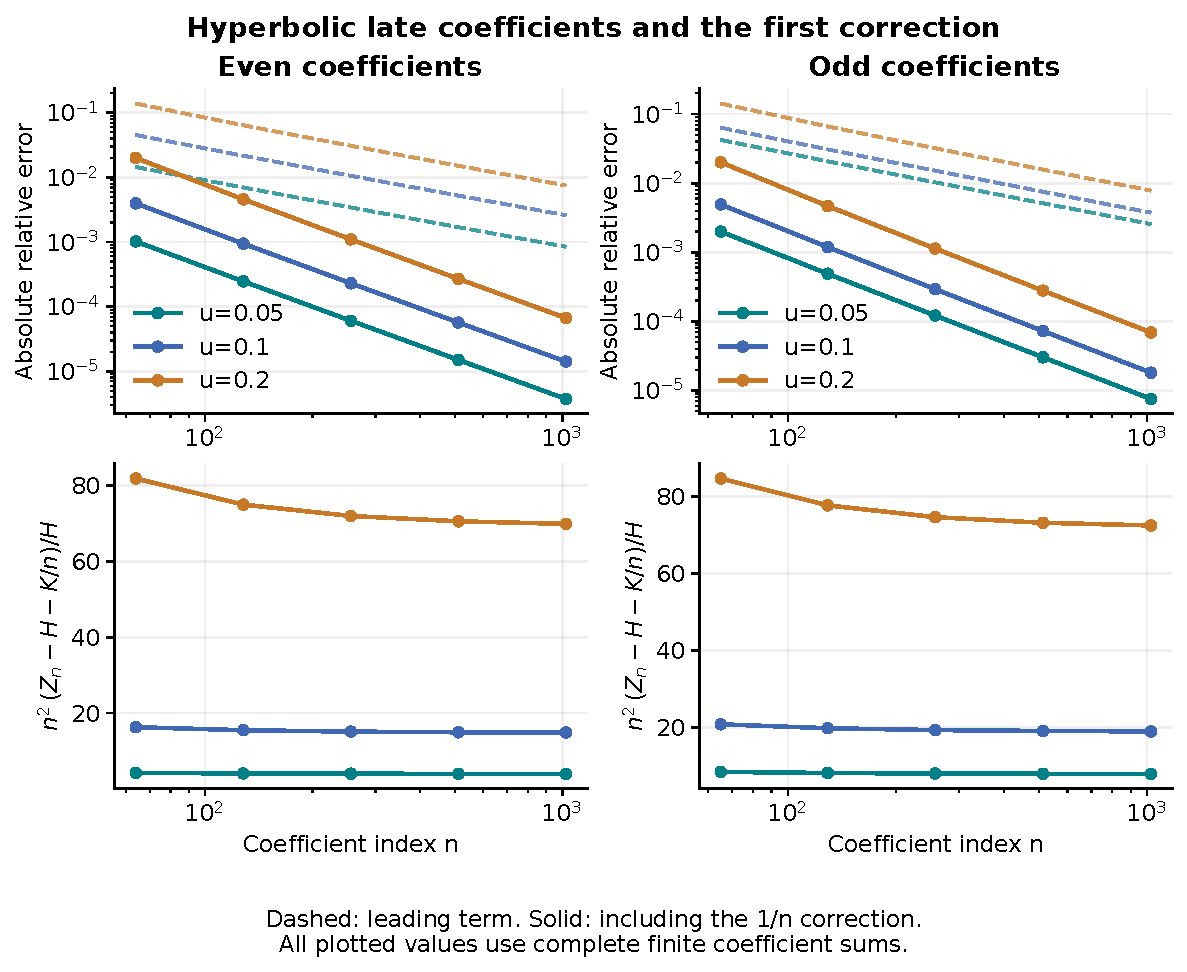
\includegraphics[width=\textwidth]{verification/asymptotic_errors.pdf}
\caption{Executed finite-sum diagnostics from the supplied program.
The observed first- and second-order decay agrees with the proved
uniform expansion. The plot is evidence of implementation consistency,
not a proof of an asymptotic estimate.}
\label{fig:errors}
\end{figure}

At the largest even and odd indices, the first correction reduces the
observed errors by factors between 37 and 592 over the tested parameters.
The recorded software versions, precision checks, full CSV, and
machine-readable results make this comparison reproducible. No interval
certification of the floating-point output is claimed.

\FloatBarrier
\section{Source audit and proposed repository integration}
\label{sec:audit}

\subsection{The inspected snapshot and the limits of the audit}

All repository references in this contribution are pinned to commit
\begin{center}
\texttt{8f5afd4d7565df808359f6a0c22f87f79a119bb9}
\end{center}
dated 12 October 2026. The research used the Polylogarithms and
Transseries indexes, relevant source chapters, and the three incoming
research archives listed below. The package's \texttt{provenance.json}
records exact paths and cryptographic hashes.

\begin{enumerate}
 \item \texttt{Resonant\_Lambert\_Inverse\_Transseries\_2026-10-12.zip}:
 the principal predecessor, including its inverse-coefficient theorem,
 exact completion and Stokes transport, and explicit research questions.
 \item \texttt{ProveIt\_Lambert\_Polylog\_Order\_Jets\_2026-10-12.zip}:
 order derivatives, resonant jets, and the arithmetic Lambert interface.
 \item \texttt{ProveIt\_Quadratic\_Polylog\_Boundaries\_2026-10-12.zip}:
 the quadratic feedback problem and its boundary regimes.
\end{enumerate}

The related integrated chapters are
\nolinkurl{01-resonant-jets.tex}, \nolinkurl{01-lambert-moments.tex}, and
\nolinkurl{01-quadratic-feedback.tex} under the Polylogarithms manuscript.
The related Transseries reports include
\nolinkurl{Polylogarithm_Resonance_And_Inverse_Transseries},
\nolinkurl{Quadratic_Polylogarithm_Feedback_Boundary_Completion}, and
\nolinkurl{Resonant_Polylogarithm_Transseries}.
In particular, the last report already proves an arbitrary-order
Fermi--Dirac Borel completion. We do not present that existing result
as a new contribution.

No specific false theorem was established in this scoped audit.
The unproved hyperbolic amplitudes are explicitly labelled conjectural
in their source; its coarser coefficient bound is valid for the purpose
there. Resolving that conjecture is an addition to the source, not a
retroactive claim that its proof was incorrect. This audit does not
certify every file in either research program.

\subsection{Concrete updates supported by the present proofs}

The following integration changes are justified without expanding the
claims beyond what is proved.

\begin{enumerate}
 \item \textbf{Promote the two amplitude conjectures.}
 In Section 11.1 of the principal predecessor, replace the conjectural
 status of \texttt{eq:conj-even} and \texttt{eq:conj-odd} by a reference
 to Theorem~\ref{thm:main}. State uniformity on $0<u\le U$ and preserve
 the distinction between coefficient index and physical target size.
 The first correction can be added as a separate strengthening.

 \item \textbf{Sharpen the inverse Borel conclusion.}
 The source's radius argument is strengthened by
 Theorem~\ref{thm:Borel-models}: both nearest real actions are genuine
 singularities for every fixed complex $u\ne0$. Include the explicit
 logarithmic and logarithmic--dilogarithmic models, with their stated
 boundary regularity.

 \item \textbf{Resolve the continuation part of Section 11.2.}
 Cite Theorem~\ref{thm:inverse-continuation} and the original closure
 theorem of Sauzin. Formulate the allowed set as $A\Z$, including the
 possibility of a singular origin on another sheet. Leave the exact
 active lattice and full local or alien description as research questions.

 \item \textbf{Retain the formal and analytic distinctions.}
 A zero-radius sector series is not made convergent by inserting
 $u=1/X$. The sectorial inverse is provided by summation as in
 Theorem~\ref{thm:inverse-summability}. Also retain the explicit
 $-t/4$ term when translating the source's degree-two remainder to the
 convention of this article; omitting it removes the amplitude shift.
\end{enumerate}

The accompanying \texttt{INTEGRATION.md} gives suggested destination
paths, stable theorem labels, and reviewable replacement prose. It
proposes a new report directory under \nolinkurl{Analysis/Transseries}
and a cross-reference from Polylogarithms. No existing source file is
silently replaced, and this package does not contain a repository push.

\section{Further research questions}
\label{sec:research}

The proofs isolate several concrete next steps. We separate problems
that appear approachable by extending the present coefficient argument
from those requiring additional analytic machinery.

\subsection{All inverse-index orders and higher boundary regularity}

Can one prove, for each fixed $N$, a locally uniform expansion
\[
 \frac{(-1)^{n+1}A^nC_n(u)}{4ub_n}
 =\sum_{j=0}^{N-1}\frac{K_{\epsilon,j}(u)}{n^j}
                  +O_{U,N}(n^{-N}),\qquad \epsilon=n\bmod2,
\]
with $K_{\epsilon,0}=H_\epsilon(cu)$ and
$K_{\epsilon,1}=K_\epsilon(u)$?
The expected route is to retain all configurations with a fixed small
total excess away from the large index, expand the gamma ratios and
$T_{n,k}$ to the same order, and bound the remainder uniformly before
summing over $k$. An explicit recursion for the resulting polynomial
coefficients multiplying $\cosh(cu)$ and $\sinh(cu)$ would be more useful
than isolated higher-order formulas.

Such a theorem would produce Borel models built from
$\Li_1,\ldots,\Li_N$, where $\Li_1(w)=-\log(1-w)$, with a
$C^{N-1}$ remainder on the closed disk. More precisely, keeping the
terms $j=0,\ldots,N-1$ above leaves Borel coefficients
$O(A^{-n}n^{-N-1})$, whose derivatives through order $N-1$ converge
absolutely on the boundary. Smooth boundary control of every finite
order would still not, by itself, identify a complete local analytic
singularity type.

\subsection{A paired-action factorial calculus}

The finite-phase theorem proves the leading transformation law
\[
 \kappa_\omega\longmapsto
 \kappa_\omega e^{\lambda_\omega\rho u},\qquad
 \lambda_\omega=A/\omega.
\]
Can the factorial asymptotic calculus of \cite{Borinsky2018} be extended
in a form that handles several equal-modulus actions and cancellations
uniformly in a parameter? For the present model one seeks simultaneous
coefficient expansions in
$\Gamma(n-1-j)A^{-(n-1-j)}$ and
$\Gamma(n-1-j)(-A)^{-(n-1-j)}$, with a rigorously justified
composition rule.
That result should reproduce Theorem~\ref{thm:main} and explain which
finite forward coefficients control each successive order. It would
also apply to root-of-unity twists and character-weighted Lambert sums.

\subsection{Which arithmetic lattice points are active?}

Theorem~\ref{thm:inverse-continuation} confines possible singularities to
$A\Z$, and Theorem~\ref{thm:Borel-models} proves activity at $\pm A$.
Determine the singular behavior at $\pm2A,\pm3A,\ldots$ on specified
continuation paths. At $2A$, for example, the forward divisor weight
$d(2)$ can interact with two nonlinear contributions of action $A$.
The problem is to separate these sources without double counting and
to decide whether any cancellations occur for special $u$.
A precise result should specify the sheet, path convention, and local
coordinate at every action.

\subsection{The full local singularity and Stokes operator}

The continuous and continuously differentiable boundary remainders do
not determine a complete analytic singularity type. Can one show that
the primitive-action singularities admit a logarithm times a convergent
or explicitly resurgent germ, and compute that germ to all orders?
The exact analytic transport in Section~\ref{sec:Stokes} gives a strong
constraint but is not a substitute for a local Borel theorem.
Care is needed at the origin on other sheets: differentiation in the
coordinate-inversion proof can change the order of a pole. A global
claim of \emph{simple resurgence} needs a separate proof.

\subsection{A growing slow parameter and a new saddle regime}

The present bounds are uniform on every fixed disk in $u$, with no
lower bound. They are not uniform as $|u|\to\infty$.
The leading exponential sum favors $k$ of size approximately $|cu|$.
When $u=u_n$ grows with $n$, both the gamma-ratio correction
$k^2/n$ and the feedback correction $uk^2/n$ can become significant.
Identify the largest growing ranges that still admit relative
hyperbolic asymptotics, and determine the transition law when the
feedback correction is order one. The size of the relative correction
$K_\epsilon(u)/(nH_\epsilon(cu))$
suggests a positive-real transition near $u$ of order $n^{1/3}$;
this is a scaling heuristic, not a theorem.

\subsection{Optimal truncation for the physical inverse}

For fixed $u$, the ratio of successive coefficient magnitudes suggests
optimal sector truncation near $n=A/|q|$, modulo the parity amplitudes.
The physical problem couples $q=e^{\gamma-X}$ and $u=1/X$, placing
that truncation order far beyond polynomial size in $X$.
Can one obtain a sharp remainder for the real inverse after optimal
truncation, together with a terminant description of the lateral jump?
The uniform coefficient theorem supplies necessary late-term data;
such a remainder theorem also needs analytic estimates on the summed
inverse and its Stokes neighborhoods.

\subsection{Moving away from exact resonance}

The incoming work contains parameter jets at exact polylogarithmic
resonance. Extend the present result to nonzero order displacement
$\varepsilon$, with coefficient bounds uniform as
$\varepsilon\log(1/q)$ changes size. The coalescing-pole core depends on
this combined variable, and its order jets contain logarithms; the
regular forward coefficients also vary with $\varepsilon$. In the
source's normalization, for $n\ge2$ and $\varepsilon$ near zero,
\[
 r_n(\varepsilon)=
 \frac{2\{1+(-1)^n\cos(\pi\varepsilon)\}}{A^n n!}
 \Gamma(n-\varepsilon)\Gamma(n+\varepsilon)
 \zeta(n-\varepsilon)\zeta(n+\varepsilon).
\]
Thus an odd regular tail is already activated away from resonance, as
proved in \cite{incoming}. The new target is a uniform theorem for the
late \emph{inverse} coefficients, specifying when this mechanism and
nonlinear odd-sector production reinforce or cancel one another, with
the corresponding action amplitudes.

\subsection{Exact verification and reusable formal components}

The finite coefficient formula, valuation identities, and the
reciprocal-binomial convolution bounds are natural candidates for
proof-assistant formalization. They involve finite algebra and
inequalities before any analytic continuation is introduced.
A separate numerical project could replace the diagnostic arithmetic
by interval bounds for selected large-index coefficients and for the
sectorial inverse. Neither task should be confused with the other:
finite exact computations check an implementation, whereas a
formalized uniform convolution theorem would certify the step that
turns all finite coefficients into an asymptotic result.

\begin{thebibliography}{20}
\small
\setlength{\parskip}{0pt}
\setlength{\itemsep}{5pt}
\raggedright
\bibitem{incoming}
\emph{Double Resonance and Nested Stokes Geometry in Polylogarithmic Lambert
Inversion}, research report prepared for Vladimir Reshetnikov / ProveIt,
12 October 2026. Source member
\nolinkurl{Resonant_Lambert_Inverse_Transseries/article.tex} in
\nolinkurl{Resonant_Lambert_Inverse_Transseries_2026-10-12.zip};
especially Sections 7, 8, and 11.1--11.2. Inspected at ProveIt commit
\texttt{8f5afd4d7565df808359f6a0c22f87f79a119bb9}.
\url{https://github.com/VladimirReshetnikov/ProveIt/blob/8f5afd4d7565df808359f6a0c22f87f79a119bb9/docs/incoming/Resonant_Lambert_Inverse_Transseries_2026-10-12.zip}.

\bibitem{DK2021}
D. Dorigoni and A. Kleinschmidt,
\emph{Resurgent expansion of Lambert series and iterated Eisenstein integrals},
Communications in Number Theory and Physics \textbf{15} (2021), 1--57.
\url{https://arxiv.org/abs/2001.11035}.

\bibitem{BD2026}
D. Broadhurst and D. Dorigoni,
\emph{Resurgent Lambert series from Feynman and beyond},
arXiv:2607.14020 (2026).
\url{https://arxiv.org/abs/2607.14020}.

\bibitem{BR1984}
E. A. Bender and L. B. Richmond,
\emph{An asymptotic expansion for the coefficients of some power series II:
Lagrange inversion}, Discrete Mathematics \textbf{50} (1984), 135--141.
\url{https://doi.org/10.1016/0012-365X(84)90043-8}.

\bibitem{Borinsky2018}
M. Borinsky,
\emph{Generating asymptotics for factorially divergent sequences},
Electronic Journal of Combinatorics \textbf{25}(4) (2018), P4.1.
\url{https://doi.org/10.37236/5999};
\url{https://arxiv.org/abs/1603.01236}.

\bibitem{Sauzin2015}
D. Sauzin,
\emph{Nonlinear analysis with resurgent functions},
Annales scientifiques de l'\'Ecole Normale Sup\'erieure, S\'erie 4,
\textbf{48}(3) (2015), 667--702. In particular Theorems 3, 5, $3'$, and $5'$.
\url{https://doi.org/10.24033/asens.2255};
\url{https://arxiv.org/abs/1212.4477}.

\bibitem{DLMF}
NIST Digital Library of Mathematical Functions,
Sections 5.7, 25.4, and 25.12: Gamma expansions, zeta reflection, and
polylogarithms. Accessed 12 October 2026.
\url{https://dlmf.nist.gov/5.7};
\url{https://dlmf.nist.gov/25.4};
\url{https://dlmf.nist.gov/25.12}.

\bibitem{repo}
V. Reshetnikov and ProveIt Contributors,
\emph{ProveIt}, Polylogarithms and Transseries research programs.
Snapshot \texttt{8f5afd4d7565df808359f6a0c22f87f79a119bb9},
12 October 2026. The inspected paths are listed in Section~\ref{sec:audit}.
\url{https://github.com/VladimirReshetnikov/ProveIt/tree/8f5afd4d7565df808359f6a0c22f87f79a119bb9/Analysis/Polylogarithms};
\url{https://github.com/VladimirReshetnikov/ProveIt/tree/8f5afd4d7565df808359f6a0c22f87f79a119bb9/Analysis/Transseries}.
\end{thebibliography}

\end{document}
